\documentclass[12pt,letterpaper,noanswers]{exam}
%\usepackage{color}
\usepackage[usenames,dvipsnames,svgnames,table]{xcolor}
\usepackage[margin=0.9in]{geometry}
\renewcommand{\familydefault}{\sfdefault}
\usepackage{multicol}
\pagestyle{head}
\usepackage{hyperref}
\definecolor{c07}{HTML}{BBFFBB}
\definecolor{c08}{HTML}{BBFFFF}
\definecolor{c09}{HTML}{BBDDFF}
\definecolor{c10}{HTML}{BBBBFF}
\definecolor{c11}{HTML}{DDBBFF}
\definecolor{c12}{HTML}{BBBBDD}
\newcommand{\mb}[1]{\underline{#1}}

\header{AM 22b Problem Set 03}{}{Due Thurs Feb 25th at 6pm ET}
\runningheadrule
\headrule
\usepackage{diagbox}
\usepackage{graphicx} % more modern
%\usepackage{subfigure} 
\usepackage{amsmath} 
\usepackage{amssymb} 
%\usepackage{gensymb} 
%\usepackage{natbib}
\usepackage{hyperref}
%\usepackage{enumitem}
%\setlength{\parindent}{0pt}
%\usepackage{setspace}
%\pagestyle{empty}  
%\newcommand{\Sc}[0]{
%{\color{BlueViolet}\S}
%}
\usepackage{tcolorbox}

\begin{document}
 \pdfpageheight 11in 
  \pdfpagewidth 8.5in
  
\begin{itemize}
    \item Review sections \S 14.1-\S 14.6, \S 16.1-2 in Hughes-Hallett, the course text.
    \item The odd numbered problems in the Exercise sections (the first chunk of problems) in each section are worthwhile practice for before a problem set.  \emph{Answers are in the back for odd numbered problems, and solutions are in the student solutions manual is available in Cabot.}
    \item The `Check your understanding' or `Strengthen your understanding' questions are a great way to check whether you're building intuition for course concepts. % Take a look at these for sections \S 12.1 - \S 12.5 (the sections we worked on last week).
\end{itemize}

\begin{questions}
\question Log in to WeBWorK and complete the problems assigned there under pset03.


\question The cardiac output, $c$, is the volume of blood flowing through a person's heart per unit time.  The systemic vascular resistance (SVR), $s$, is the resistance to blood flow in the veins and arteries.  Let $p$ be a person's blood pressure.  \[p=f(c,s).\]
\begin{parts}
\item What does the instantaneous rate of change $\displaystyle\frac{\partial p}{\partial c}$ represent?
\begin{solution}
This is the instantaneous rate of change of the blood pressure with respect to change in the cardiac output when the resistance to blood flow is held constant.
\end{solution}
\item Suppose that $p$ is proportional to $c$ and to $s$, so $\displaystyle p = k c s$.  Create a contour plot in Matlab for the case $k = 1.$


Use the \texttt{'LevelList'} option to set the levels of the contours.
For your plot, add labels, thicken your contour lines so that they are visible, add a title, and adjust the font size on the axes so that it is at least 14.

What do these level curves represent in the context of this problem?
\begin{solution}
The level curves show all of the combinations of cardiac output and vascular resistance that lead to a particular blood pressure.

\begin{verbatim}
fcontour(c*s,[0 8 0 8],'linewidth',3,'levellist',2:2:10)
hold on
axis equal
xlabel('c');ylabel('s');
set(gca,'FontSize',14)
plot(2,2,'r.','Markersize',20)
text(2,2.2,'A','fontsize',14)
plot(3,4/3,'r.','Markersize',20)
text(3,4/3+0.2,'B','fontsize',14)
title({'blood pressure as a function of',...
'cardiac output and vascular resistance'})
\end{verbatim}

\includegraphics[width=4in]{img/pset04p1.jpg}

\end{solution}
%\item   For $p = k c s$ (with $k$ an unknown constant), sketch four level curves of $p$, labeling each curve, your axes, and your scales (some of these labels will depend on $k$).  

\item For a person with a weak heart, it is desirable to have the heart pump against less resistance while maintaining the same blood pressure.  Such a person may be given the drug nitroglycerine to decrease the systemic vascular resistance, and the drug dopamine to increase the cardiac output.  Add this scenario to your contour plot (within Matlab) by marking a point $A$ that represents the person's state before drugs are administered and a point $B$ for their state after.

The command \texttt{plot(3,2,'k.','MarkerSize',10)} will place a black dot at the point $(3,2)$.  The command \texttt{text(3,2.2,'A','fontsize',14)} will place the letter ``A'' at the point $(3,2.2)$ (to act as a label).

\item After a heart attack a patient's cardiac output drops, causing blood pressure to drop.  The text says ``a common mistake made by medical residents is to get the patient's blood pressure back to normal by using drugs to increase the SVR, rather than by increasing the cardiac output''.  

Using Matlab, add points $D$, $E$, and $F$ to your contour diagram to show this scenario.  Choose $D$ for the patient before the heart attack, $E$ for the patient immediately after the heart attack, and $F$ after the patient has been given drugs to increase the SVR.

\emph{Make sure to choose a point $D$ where increasing SVR is the wrong thing to do.}
\end{parts}


\question Two surfaces can be said to be \emph{tangential} at a point $(a,b,c)$ if they have the same tangent plane at that point.  In this problem, you'll find all points in $3$-space where the two surfaces $z = \sqrt{2x^2+2y^2-16}$ and $z = \frac{1}{4}(x^2+y^2)$ are tangential.
\begin{parts}
\item Graph the two surfaces in matlab.  Use transparency (the \texttt{'FaceAlpha'} option in \texttt{fsurf}) to make the surfaces more visible.

Label your axes, adjust the font size, and give your plot a title.  Use the rotation tool to explore the surfaces.  I found the tangency was very visible in my plot.

Submit the graph as part of your problem set.  You do not need to submit this code on Gradescope.
\begin{solution}
\begin{verbatim}
hold off
syms x y
f = @(x,y) sqrt(2*(x^2+y^2)-16);
g = @(x,y) (x^2+y^2)/4;
domain = [-5 5 -5 5];
fsurf(x,y,f(x,y),domain,'facealpha',0.8,'edgecolor','none')
hold on
fsurf(x,y,g(x,y),domain,'facealpha',0.8,'edgecolor','none')
axis equal
xlabel('x'); ylabel('y'); zlabel('z')
set(gca,'FontSize',14)
hold on
syms t
fplot3(4*cos(t),4*sin(t),sym(4),[0 2*pi],'linewidth',3)
title('surfaces with their tangent curve')
\end{verbatim}

\includegraphics[width=5in]{img/pset04p3.jpg}
\end{solution}
\item Find the set of points where the surfaces are tangential.

\emph{It may be helpful to think of $z = \sqrt{2x^2+2y^2-16}$ as the surface $2x^2 + 2y^2 - z^2 = 16.$}
\begin{solution}
Our two surfaces can be given by $F(x,y,z) = 2x^2+2y^2 - z^2 = 16$, so the $16$-level set of $F(x,y,z)$, and by $G(x,y,z)=\frac{1}{4}(x^2+y^2)-z = 0$.

The two surfaces will have the same tangent plane at a point if the surfaces intersect at the point and have the same normal vector directions at the point.

To think about intersections, let $r^2 = x^2+y^2$, so $2r^2 - z^2 = 16$ and $\frac{1}{4}r^2 - z = 0$.  Rearranging each, $r^2 = \frac{1}{2}z^2 + 8$ and $r^2 = 4z$.  These surfaces will intersect when $4z = \frac{1}{2}z^2 + 8 \Rightarrow z^2 - 8z + 16 = 0$.  This is $(z-4)^2 = 0$ so they intersect when $z = 4$.  For $z = 4$, we have $r^2 = 4z$ so $r^2 = 16$.

The points of intersection are points $(x,y,z)$ such that $x^2+y^2 = 16$ and $z = 4$.

Now we want to determine whether the surfaces have parallel normal vectors at these points.  The normal vectors are $\vec \nabla F = \langle 4x, 4y, -2z\rangle$ and $\vec\nabla G = \langle \frac{1}{2}x, \frac{1}{2}y, -1\rangle.$  Plugging in $z = 4$ we have $\vec\nabla F = \langle 4x, 4y, -8\rangle$.  This $\vec k$ component is clearly $8$ times the $\vec\nabla G$ $\vec k$ component.  $\frac{1}{8}\vec\nabla F = \langle \frac{1}{2}x , \frac{1}{2}y , -1\rangle = \vec\nabla G$ so the vectors are parallel.

Since the surfaces intersect and have parallel normal vectors when $z =4, x^2+y^2 = 16$, the two surfaces are tangential on that circle of points.
\end{solution}
\item Check your work by showing (algebraically) that the each point you've identified satisfies the equation for each surface.

\begin{solution}
I'll plug in $x^2+y^2 = 16$ to each equation and check that $z = 4$ is a solution given the constraint on $x$ and $y$.  $z = \sqrt{2(16)-16} = \sqrt{16} = \pm 4$ so $z = 4, x^2+y^2 = 16$ is a set of solutions.

$z = \frac{1}{4}(16) = 4$ so $z=4,x^2+y^2 = 16$ is a solution here as well.  The points I've identified sit on both surfaces.
\end{solution}
\item In addition, confirm that the surfaces have the same tangent plane at each point in your set.  \emph{Explicitly showing this mathematically is great.  However, it is sufficient to explain how you know that you've found the tangent planes, and that they are identical.}
\begin{solution}
The tangent plane at $(a,b,c)$ for $F(x,y,z) = 16$ is \[4a(x-a) + 4b(y-b) -8(z-c) = 0. \]  The tangent plane at $(a,b,c)$ for $G(x,y,z) = 0$ is \[\frac{a}{2}(x-a) + \frac{b}{2}(y-b) -(z-c) = 0.\]  The left hand sides differ by a factor of $8$ but because the right hand side is zero, these are the same plane.
\end{solution}
\end{parts}


\question Let $x = r\cos\theta$, $y=r\sin\theta$, so $r = \sqrt{x^2+y^2}$ and for $x>0, y>0, \theta = \arctan(y/x)$. This is the polar coordinate system.  It is common to need to move back and forth between Cartesian coordinates and polar coordinates depending on which coordinate system is more convenient to use for a particular problem.  The chain rule allows us to relate partial derivatives in one coordinate system to partial derivatives in the other.


Let $z= f(x,y)$.  Show your mathematical steps for the work below.
\begin{parts}
\part Let $\mb{u} = \left(\begin{array}{c}r \\ \theta \end{array}\right)$.  Let $\mb{w} = \left(\begin{array}{c}x \\ y \end{array}\right)$.  Find the Jacobian matrix $\displaystyle\frac{\partial \mb{w}}{\partial \mb{u}}$.
\item  We have $\displaystyle\frac{\partial z}{\partial\mb{u}} = \left[\partial z/\partial r,  \partial z/\partial\theta\right]$ and $\displaystyle\frac{\partial z}{\partial\mb{w}} = \left[\partial z/\partial x,  \partial z/\partial y\right]$. Use the chain rule and $\displaystyle\frac{\partial \mb{w}}{\partial \mb{u}}$ to write $\partial z/\partial r$ and $\partial z/\partial\theta$ in terms of $\partial z/\partial x$ and $\partial z/\partial y$, $r$, and $\theta$.
\begin{solution}
We have \[\frac{\partial z}{\partial r} = \frac{\partial z}{\partial x}\frac{\partial x}{\partial r}+\frac{\partial z}{\partial y}\frac{\partial y}{\partial r}.\]
Similarly, \[\frac{\partial z}{\partial \theta} = \frac{\partial z}{\partial x}\frac{\partial x}{\partial \theta}+\frac{\partial z}{\partial y}\frac{\partial y}{\partial \theta}.\]

We don't know the function $f(x,y)$ so we can't simplify the partials of $z$.  However, we do know $x(r,\theta)$ and $y(r,\theta)$.  We have

$x_r = \cos \theta$

$y_r = \sin \theta$

$x_\theta = -r\sin\theta$

$y_\theta = r\cos\theta$.

Substituting,
 \[\frac{\partial z}{\partial r} = \frac{\partial z}{\partial x}\cos\theta+\frac{\partial z}{\partial y}\sin\theta.\]
 \[\frac{\partial z}{\partial \theta} = \frac{\partial z}{\partial x}r(-\sin\theta)+\frac{\partial z}{\partial y}r\cos\theta = r\left(-\frac{\partial z}{\partial x}\sin\theta+\frac{\partial z}{\partial y}\cos\theta\right).\]
\end{solution}
\part Find $z_x$ and $z_y$ in terms of $z_r$, $z_{\theta}$, $r$, and $\theta$.  There are two ways to do this:
\begin{itemize}
    \item Find $\partial\mb{u}/\partial\mb{w}$ and use the chain rule.
    \item Multiply your $z_r$ equation from (b) by $\cos\theta$ and your $z_{\theta}$ equation by $-\frac{1}{r}\sin\theta$.  Then sum the two equations and simplify to find an expression for $z_x$ in terms of $z_r$ and $z_{\theta}$.  Do something similar to isolate $z_y$.
\end{itemize}


\begin{solution}
We are told to multiply the $z_r$ equation by $\cos\theta$, so we have
 \[\frac{\partial z}{\partial r}\cos\theta = \frac{\partial z}{\partial x}\cos^2\theta+\frac{\partial z}{\partial y}\cos\theta\sin\theta.\]
 Similarly, we are told to multiply the $z_\theta$ equation by $-\frac{1}{r}\sin\theta$, so we have
  \[-\frac{1}{r}\frac{\partial z}{\partial \theta}\sin\theta = -\frac{1}{r}r\left(-\frac{\partial z}{\partial x}\sin^2\theta+\frac{\partial z}{\partial y}\cos\theta\sin\theta\right)
  = \frac{\partial z}{\partial x}\sin^2\theta-\frac{\partial z}{\partial y}\cos\theta\sin\theta.\]
  
  Next we're asked to sum the two equations and simplify, so we have
   \[\frac{\partial z}{\partial r}\cos\theta-\frac{1}{r}\frac{\partial z}{\partial \theta}\sin\theta = \frac{\partial z}{\partial x}\cos^2\theta+\frac{\partial z}{\partial y}\cos\theta\sin\theta+\frac{\partial z}{\partial x}\sin^2\theta-\frac{\partial z}{\partial y}\cos\theta\sin\theta.\]
   Rearranging, this is
     \[\frac{\partial z}{\partial r}\cos\theta-\frac{1}{r}\frac{\partial z}{\partial \theta}\sin\theta =\frac{\partial z}{\partial x}(\cos^2\theta+\sin^2\theta).\]
     Since $\cos^2\theta + \sin^2\theta = 1$ we have
     \[\frac{\partial z}{\partial x} = \frac{\partial z}{\partial r}\cos\theta-\frac{1}{r}\frac{\partial z}{\partial \theta}\sin\theta.\]

\end{solution}
\part Show that \[\left(\frac{\partial z}{\partial x}\right)^2+\left(\frac{\partial z}{\partial y}\right)^2 = \left(\frac{\partial z}{\partial r}\right)^2+\frac{1}{r^2}\left(\frac{\partial z}{\partial \theta}\right)^2.\]
\begin{solution}
We use the relationships from above to show this.  We have
\begin{align*}
z_x^2+z_y^2 &= \left(\frac{\partial z}{\partial r}\cos\theta-\frac{1}{r}\frac{\partial z}{\partial \theta}\sin\theta\right)^2+\left( \frac{\partial z}{\partial r}\sin\theta +\frac{1}{r}\frac{\partial z}{\partial \theta}\cos\theta\right)^2 \\
\end{align*}

Hopefully this will simplify nicely and the expression above will fall out.

\begin{align*}
z_x^2+z_y^2 &= \left(\frac{\partial z}{\partial r}\cos\theta-\frac{1}{r}\frac{\partial z}{\partial \theta}\sin\theta\right)^2+\left( \frac{\partial z}{\partial r}\sin\theta +\frac{1}{r}\frac{\partial z}{\partial \theta}\cos\theta\right)^2 \\
&= z_r^2\cos^2\theta- \frac{2}{r}z_rz_{\theta}\cos\theta\sin\theta + \frac{1}{r^2}z_{\theta}^2\sin^2\theta + z_r^2\sin^2\theta +\frac{2}{r}z_rz_{\theta}\cos\theta\sin\theta + \frac{1}{r^2}z_{\theta}^2\cos^2\theta \\
&= z_r^2(\cos^2\theta+\sin^2\theta) + \frac{2}{r}z_rz_{\theta}(-\cos\theta\sin\theta+\cos\theta\sin\theta) + \frac{1}{r^2}z_{\theta}^2(\sin^2\theta +\cos^2\theta )\\
&= z_r^2+ \frac{1}{r^2}z_{\theta}^2,\\
\end{align*}
so we have shown that
\[z_x^2+z_y^2 = z_r^2+ \frac{1}{r^2}z_{\theta}^2,\] as desired.
\end{solution}


\end{parts}

% \item Determine, without calculation, whether the following integrals are positive, negative, or zero.  Explain your reasoning. 

% Let $D$ be the region inside the unit circle centered at the origin, let $R$ be the right half of $D$, and let $B$ be the bottom half of $D$.  

% Let $S$ be the solid region inside the sphere $x^2+y^2+z^2 = 1$ and $T$ the top half of this sphere.

% See \url{https://www.youtube.com/watch?v=i5qNz-MSwhY} for a video with two examples of this type of problem.
% \begin{parts}
% \part $\int_R 5x\ dA$
% \part $\int_B 5x\ dA$
% \part $\int_D(y-y^3)\ dA$  \emph{Note: for $\vert y\vert<1$, $\vert y^3\vert<\vert y\vert$}
% \part $\int_B(y-y^3)\ dA$
% \part $\int_T e^z\ dV$
% \part $\int_S \sin z\ dV$
% \end{parts}


\item For each of the following iterated integrals, translate the bounds of each integral into equations, and sketch the region of integration.
\begin{parts}
\item  \[\int_0^1\int_{x-2}^{\cos \pi x} y\ dy\ dx.\]
\begin{solution}
 This is the region above the curve $y=x-2$ and below the curve $y=\cos(\pi x)$ with $0\leq x\leq 1$.
 
 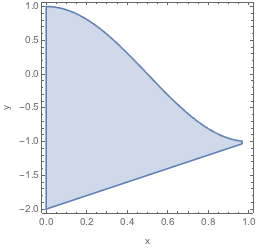
\includegraphics[width=2in]{img/HW06_r2.png}

\texttt{RegionPlot[0 <= x <= 1 \&\& x-2 <= y <= Cos[Pi x], \{x, 0, 1\}, \{y, -2, 1\}, 
 FrameLabel -> \{"x", "y"\}]}
\end{solution}

\item \[\int_0^1\int_{-1}^1\int_0^{\sqrt{1-z^2}} 3z\ dy\ dz\ dx\]
\begin{solution}
The inner bound corresponds to the inequality $0\leq y \leq \sqrt{1-z^2}$.  This implies $y^2 = 1-z^2$ is the upper bound in $y$.  Rearranging, that boundary is the circle $y^2+z^2 =1$.  Since the lower bound on $y$ is zero, we have a half disk.  The $x$ bounds are from $0$ to $1$ so that half disk becomes a half cylinder.

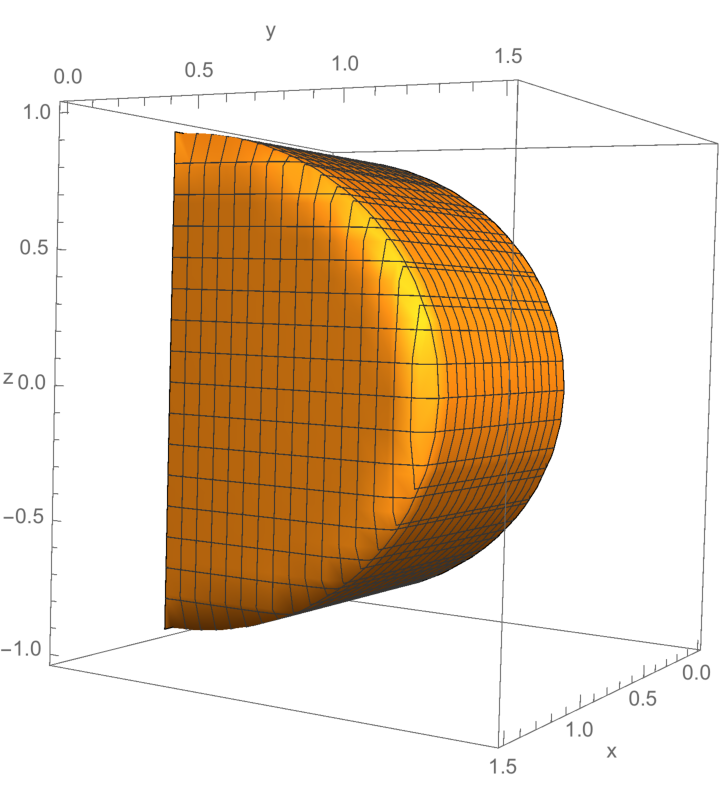
\includegraphics[width=2in]{img/HW06_r6.pdf}

\texttt{RegionPlot3D[
 0 <= x <= 1 \&\& 0 <= y \&\& y <= Sqrt[1 - z\^{}2] \&\& -1 <= z <= 1 , \{x, 0, 
  1.5\}, \{y, 0, 1.5\}, \{z, -1, 1\}, AxesLabel -> \{"x", "y", "z"\}, 
 AspectRatio -> 1]}

\end{solution}



\item \[\int_0^1\int_{-\sqrt{1-z^2}}^{\sqrt{1-z^2}}\int_0^{\sqrt{1-x^2-z^2}} \sin x\ dy\ dx\ dz.\]

\begin{solution}

The inner bounds constraint the shape.  These are $0\leq y\leq \sqrt{1-x^2-z^2}$.  The lower bound is $y=0$ so our shape is on the right side of the $xz$-plane.  We have $y = \sqrt{1-x^2-z^2} \Rightarrow x^2+y^2+z^1 = 1$ for the upper bound.  The $y$-bounds constraint us to the region inside the unit sphere and to the right of the $xz$-plane.  This is a solid hemisphere.

The outer pair of bounds describes in region in the $xz$-plane that constraints the shadow of the object.  This region is $-\sqrt{1-z^2}<x<\sqrt{1-z^2}$ and $0<z<1$.  Both $x$ bounds become $x^2+z^1 = 1$.  Since $z>0$, this is the region inside the half circle where $z$-is positive.

Combining the $y$-bound information that gives us the overall shape with our knowledge of where the shadow occurs, we have the solid region inside a quarter sphere where $y\geq 0$ and $z\geq 0$ as shown in the plot below.

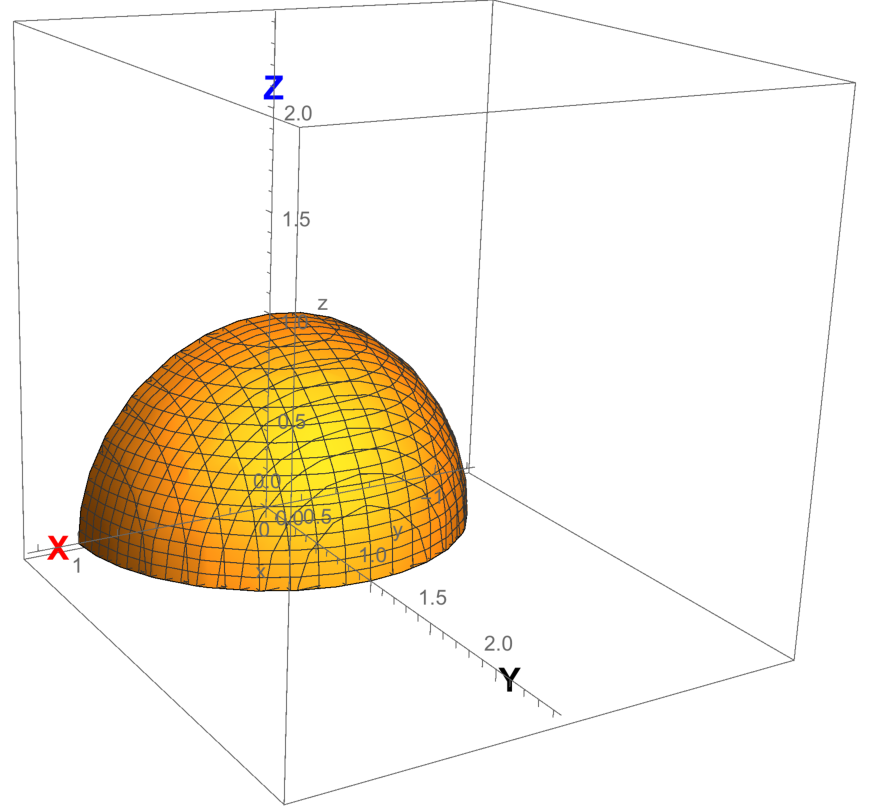
\includegraphics[width=3in]{img/HW06s1.pdf}

\begin{verbatim}
p1 = RegionPlot3D[
   0 <= z <= 1 && -Sqrt[1 - z^2] <= x <= Sqrt[1 - z^2] && 
    0 <= y <= Sqrt[1 - z^2 - x^2] , {x, -1.2, 1.2}, {y, 0, 2.4}, {z, 
    0, 2.4}, AxesLabel -> {"x", "y", "z"}, BoxRatios -> {1, 1, 1}, 
   AxesOrigin -> {0, 0, 0}];
p2 = Graphics3D[{Text[Style["X", Bold, Red, 16], {1.1, 0, 0}], 
    Text[Style["Y", Bold, Black, 16], {0, 2.1, 0}], 
    Text[Style["Z", Bold, Blue, 16], {0, 0, 2.1}]}];
Show[p1, p2]
\end{verbatim}


\end{solution}


\end{parts}

% \item For the following, identify whether the statement is true or false.  Include a justification of your choice.
% \begin{parts}
% \part If $f(x,y) = k$ for all points $(x,y)$ in a region $R$ then $\int_R f\ dA = k \cdot \text{Area}(R)$.
% \begin{solution}
% We have $\int_R k\ dA$ with $k$ a constant.  Since constants can come out of an integral, this is 
% \[\int_R k\ dA = k\int_R dA = k\cdot \text{Area}(R).\]  The statement is true.
% \end{solution}
% \part If $R$ is the rectangle $0 \leq x \leq 1, 0 \leq y \leq 2$ and $S$ is the square $0\leq x \leq 1, 0 \leq y \leq 1$, then $\int_R f\ dA = 2\int_S f\ dA$.
% \begin{solution}
% This statement is sometimes true, so is false for the purposes of this problem.  Consider the function $f = x$.  $\int_R x\ dA > 2\int_S x\ dA$ because the function is smaller on $S$ than it is on the rest of $R$.
% \end{solution}
% \part The iterated integrals \[\int_{-1}^1\int_0^1\int_0^{1-x^2}f\ dzdydx\] and \[\int_0^1\int_0^1\int_{-\sqrt{1-z}}^{\sqrt{1-z}}f\ dxdydz\] are equal.
% \begin{solution}
% The first region is given by $-1\leq x\leq 1$ and $0\leq y \leq 1$ and $0\leq z \leq 1-x^2$.  

% The second region has identical $y$ bounds (and the shapes do not vary with $y$).  This means we just need to compare whether the regions take up the same portion of the $xz$-plane.  

% In the $xz$-plane we are comparing $-1\leq x\leq 1$ and $0\leq z \leq 1-x^2$ to $0\leq z\leq 1$ and $-\sqrt{1-z}\leq x \leq \sqrt{1-z}$.

% The shape on the left is the region above $z = 0$ and below the parabola $z = 1-x^2$.  The constraints $-1\leq x\leq 1$ come from the intersection of $z=0$ and the parabola.

% The shape in the right is the region to the left of $-\sqrt{1-z} = x$, to the right of $x=\sqrt{1-z}$, and above $z=0$.  The left and right constraint curves both convert to $x^2 = 1-z \Rightarrow z = 1-x^2$.  So this is also the region above $z = 0$ and below the parabola $z= 1-x^2$.

% The region in the $xz$-plane is identical for both objects and the $y$-bounds match as well, so these integrals have the same region of integration.  They also have the same integrand, so the equality holds and the statement is true.
% \end{solution}

%\end{parts}

% \item Evaluating an integral example video: \url{https://www.youtube.com/watch?v=DgsTXYpbcu4}
% \begin{parts}
% \item Sketch the region of integration and evaluate the integral for \[\int_1^4\int_{\sqrt{y}}^y x^2y^3\ dx\ dy.\]

% \begin{solution}
% This region is $\sqrt{y}\leq x\leq y$ with $1\leq y\leq 4$.  So $x$ goes from $\sqrt{y}$ up to $y$:

% 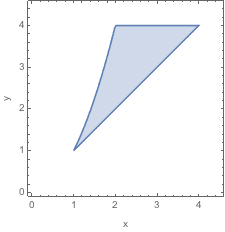
\includegraphics[width=2in]{img/HW06_r3.png}

% \texttt{RegionPlot[1 <= y <= 4 \&\& Sqrt[y] <= x <= y, \{x, 0, 4.5\}, \{y, 0, 4.5\}, 
%  FrameLabel -> \{"x", "y"\}]}
 
%  To evaluate:
%  \begin{align*}
%  \int_1^4\int_{\sqrt{y}}^y x^2y^3\ dx dy = &\ \int_1^4\frac{1}{3}y^3\left.(x^3)\right\vert_{x=\sqrt{y}}^{x=y}\ dy\\
%  =&\ \int_1^4\frac{1}{3}y^3(y^3-y^{3/2})\ dy \\
%   =&\ \frac{1}{3}\int_1^4y^6-y^{9/2}\ dy \\
%     =&\ \frac{1}{3}\left.(\frac{1}{7}y^7-\frac{2}{11}y^{11/2})\right\vert_1^4 \\
%     =&\ \frac{1}{3}(\frac{1}{7}(4^7-1)-\frac{2}{11}(4^{11/2}-1)) \\
%         =&\ \frac{1}{21}(4^7-1)-\frac{2}{33}(4^{11/2}-1) \\
%  \end{align*}
% \end{solution}

% \item For the two regions shown below, compute the integral of $f(x,y) = xy$ over the region shown.

% 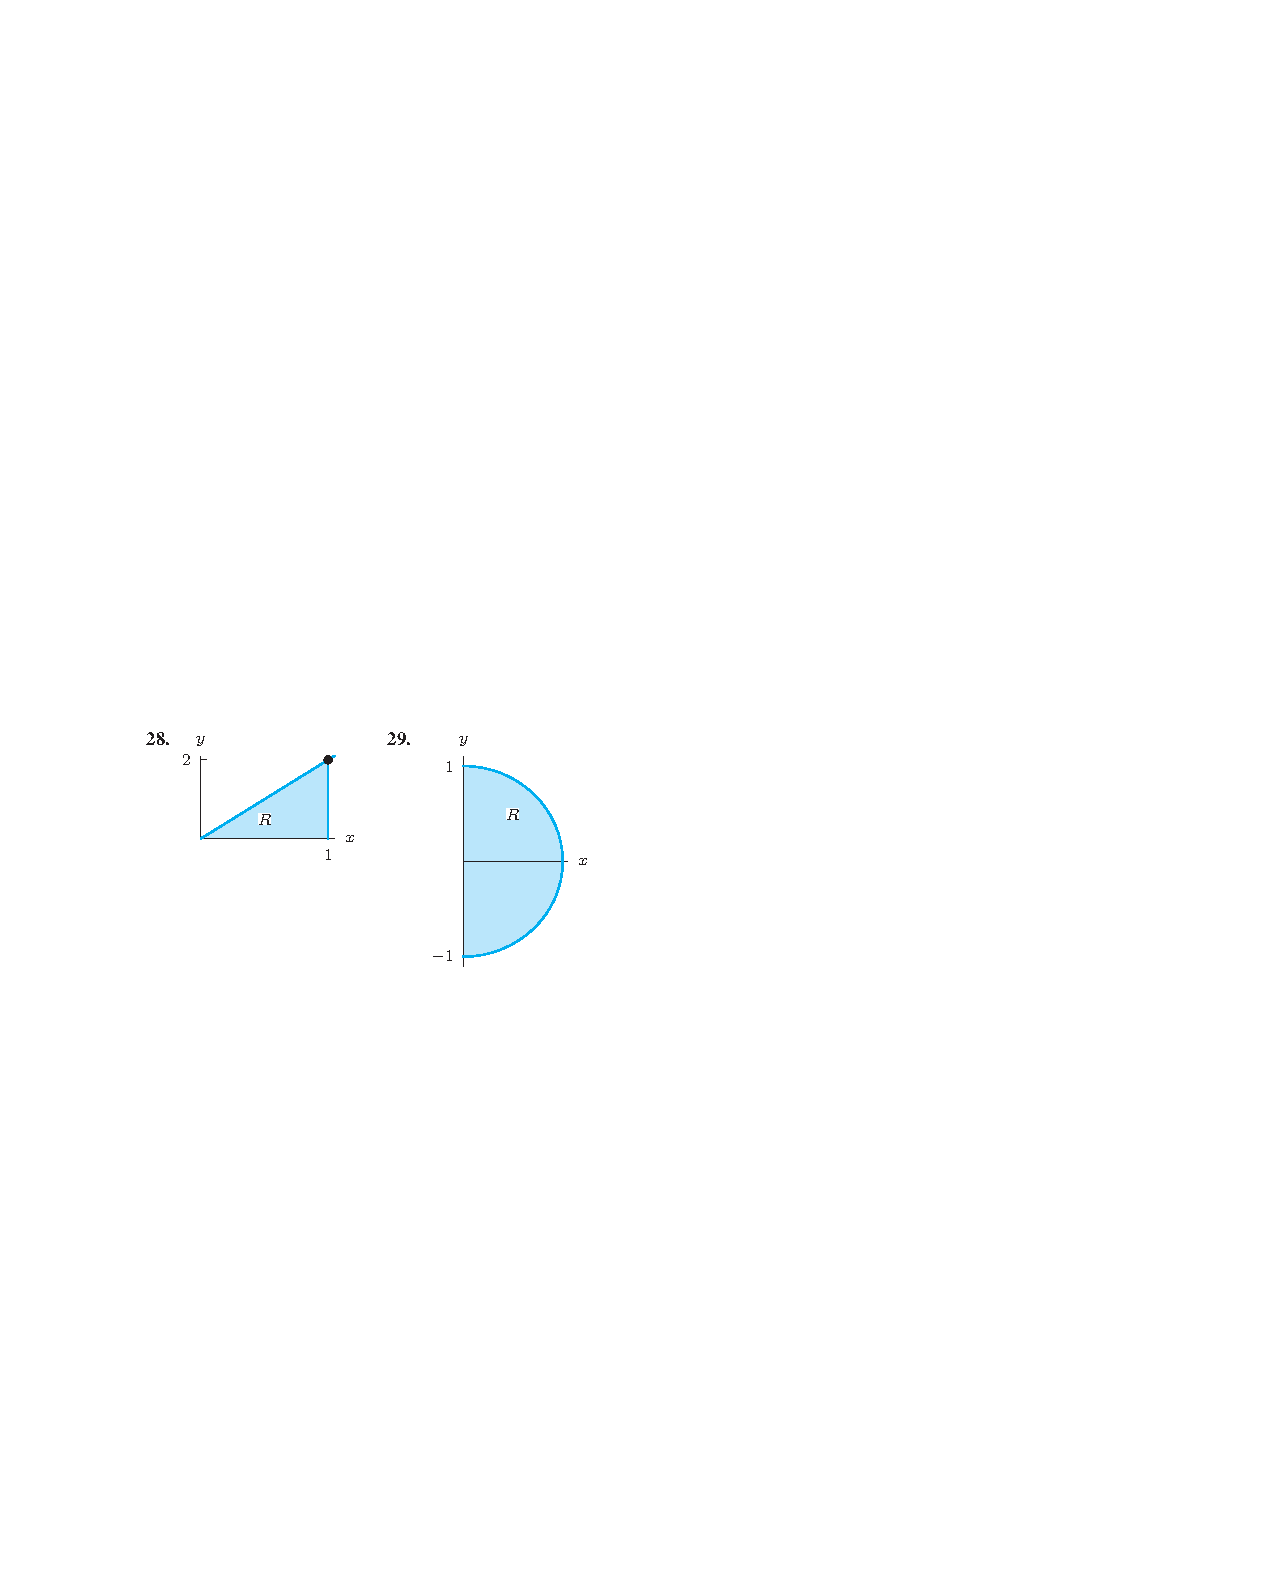
\includegraphics{img/HW06p1.pdf}

% \begin{solution}
% For the region on the left, we have $0\leq y\leq 2x$ since the bounding line goes from $(0,0)$ to $(1,2)$.  In addition, $0\leq x\leq 1$.  Setting up an integral, this is \begin{align*}
% \int_0^1\int_0^{2x} xy\ dy\ dx &= \frac{1}{2}\int_0^1 x\left(\left.y^2\right\vert_0^{2x}\right)\ dx\\
% &= \frac{1}{2}\int_0^1 x(4x^2)\ dx\\
% &=2\int_0^1 x^3\ dx\\
% &=2\frac{1}{4}\left.x^4\right\vert_0^1 \\
% &= \frac{1}{2}.
% \end{align*}

% For the region on the right, we have a symmetry.  Specifically, at a fixed value of $x$, along a line through the object, we have $y<0$ below the $x$-axis and $y>0$ above the $x$-axis, with a symmetry in the shape of the object on either side of the axis.  The interior integral of $\int_0^1x\int_{-\sqrt{1-x^2}}^{\sqrt{1-x^2}} y\ dy\ dx$ is $0$ so the integral of $xy$ over the region will be zero.
% \end{solution}

% \end{parts}

% \item Log in to WeBWorK and complete the 7 problems assigned there under HW06.  \textbf{Write up WeBWorK problems 2, 3, 4, and 5 to be turned in as part of this assignment}.  WeBWorK will grade these for correctness.  In your write-up, they will be graded for your setup and showing the steps of working through the problem.  \emph{Note: You may need to review $u$-substitutions to complete some of the integrals.}
% \begin{parts}
% \item Webwork Q2
% \item Webwork Q3
% \item Webwork Q4
% \item Webwork Q5
% \end{parts}



% \item Convert the following from polar coordinates to Cartesian coordinates or from Cartesian coordinates to polar coordinates.  Sketch each curve in the $xy$-plane.
% \begin{parts}
% \item $r=\frac{2}{\sin\theta}$.
% \begin{solution}
% This is the curve $r\sin\theta = 2$ so $y=2$.

% 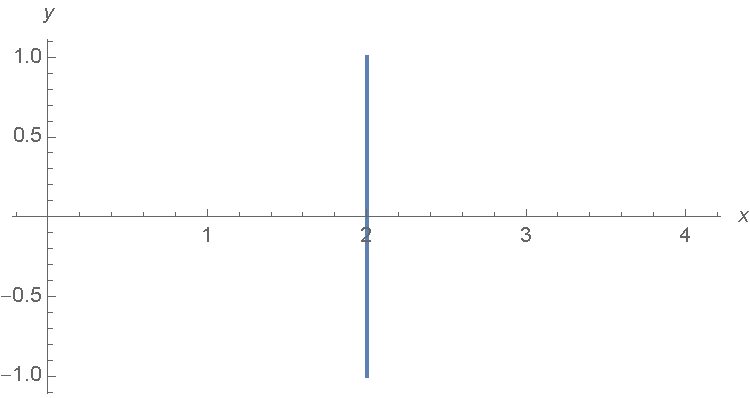
\includegraphics[width=2in]{img/HW06s5.pdf}
% \end{solution}
% \item $y=\sqrt{1-x^2}$.
% \begin{solution}
% This is the curve $y^2=1-x^2$ so $x^2+y^2  =1 \Rightarrow r = 1$.  Note that $0\leq \theta \leq \pi$, since this is just a half-circle.

% 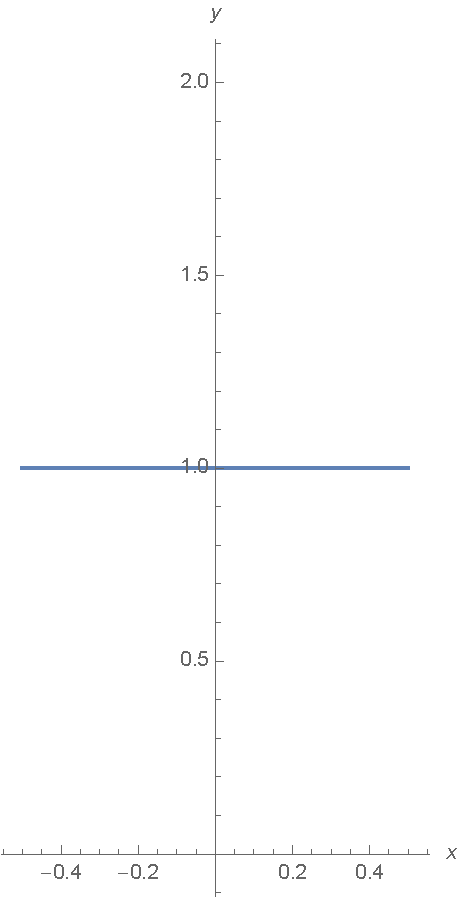
\includegraphics[width=2in]{img/HW06s4.pdf}
% \end{solution}
% \item $r=\frac{1}{\cos\theta}$.
% \begin{solution}
% This is the curve $r\cos\theta = 1$ so $x=1$.

% 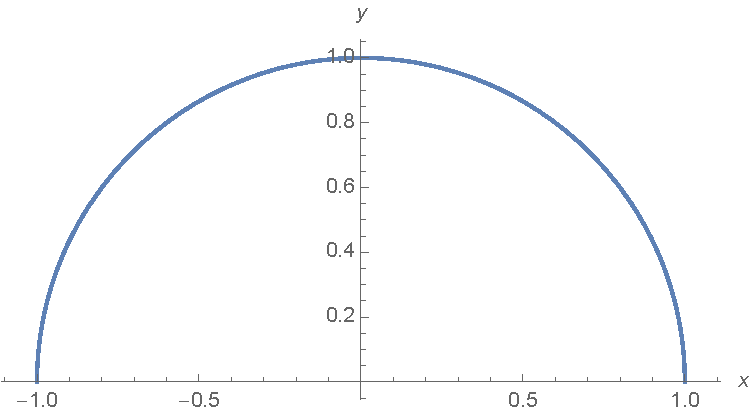
\includegraphics[width=2in]{img/HW06s3.pdf}
% \end{solution}
% \item $\theta = 3\pi/4$.
% \begin{solution}
% This is the curve along the line where $\theta = 3\pi/4$ which occurs when $y = -x$.  Note that this is only the portion where $r\geq 0$, so where $y>0, x<0$.

% 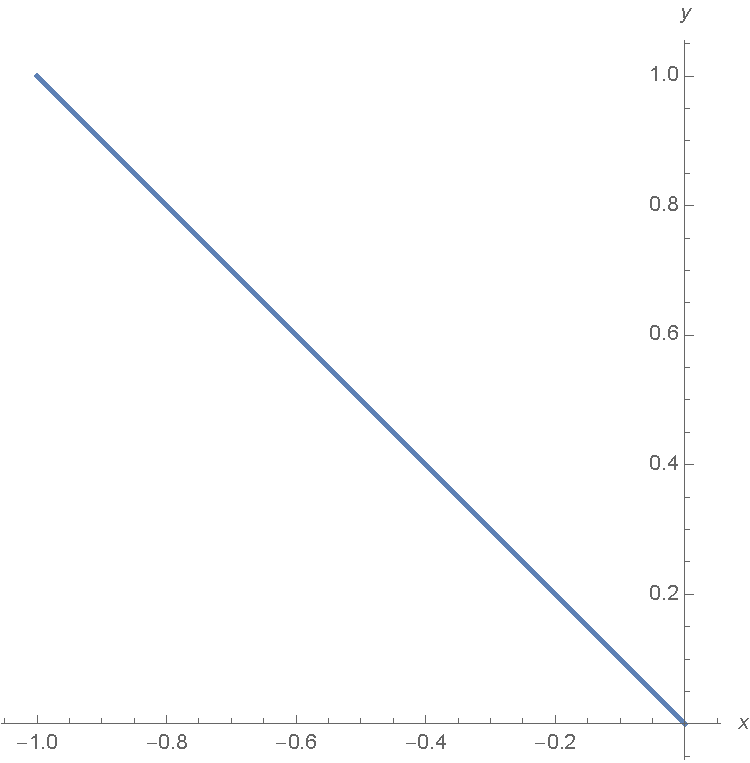
\includegraphics[width=2in]{img/HW06s2.pdf}
% \end{solution}
% \end{parts}

\question (Approximating the volume of the island of Kauai)

In \texttt{imagesKauai.mat} you'll find two elevation data sets:
\begin{itemize}
    \item \texttt{imALOS} holds the ALOS elevation data.  The elevation is in meters and each element of the matrix corresponds to a $30$ by $30$ meter box on the ground.  \texttt{infoALOS} holds the latitude and longitude extent for the image.
    \item \texttt{imUSGS} holds a USGS elevation dataset.  The elevation is in meters and each element of the matrix corresponds to a $10$ by $10$ meter box on the ground.  \texttt{infoUSGS} holds the latitude and longitude extent for the image.
\end{itemize}

\begin{parts}
\item On a single set of axes (with the horizontal axis given by longitude and the vertical axis by latitude), plot contours of both datasets.  Include axis labels and submit your plot as part of your problem set.
\item Use the ALOS data to approximate the volume (above sea level at zero meters) of Kauai.  Measure this in cubic meters.
\item Use the USGS data to approximate the volume (above sea level at zero meters) of Kauai.  Measure this in cubic meters.
\item Compute the average height of Kauai.
\item If you were to flood the state of Massachusetts with 1 meter of water, would the volume of that water be larger or smaller than the volume of Kauai?  \emph{Provide your reasoning.}
\item Submit the Matlab code that you used for (a), (b), (c), (d) as part of your problem set submission.
\end{parts}



\end{questions}

\end{document}
